
\chapter{Design and Implementation of Self Tuning PI and PID Controllers on Single Board Heater System}

\section{Introduction}%\label{hints}
This chapter presents Design and Implementation of Self Tuning PI and PID Controllers on Single Board Heater System done by Mr. Vikas Gayasen.\footnote{Copyright: Mr. Vikas Gayasen, student of Prof. Kannan Moudgalya, IIT Bombay for process control course, 2010}
When a plant is wired in a close loop with a PID controller, the parameters, $K_c$, $\tau_i$ and $\tau_d$ determine the variation of the manipulated input that is given by the controller. This, in turn, determines the variation of the controlled variable, when a set point is given. Suitable values of these parameters can be found out when plant transfer function is known. However, with large changes in the controlled variable, there may be appreciable changes in the plant transfer function itself. Therefore, it is needed to dynamically update the controller parameters according to the transfer function.

\subsection{Ojective}%\label{umlauts}
The objective of the present study was to design and implement an algorithm that would dynamically update the values of the controller parameters that are used to control the temperature in the Single Board Heater System (SBHS).



\section{Theory}
\subsection{Why a Self Tuning Controller?}
The transfer function of SBHS is assumed as 


\begin{align}
	%\Delta$T = frac {K_p}{(\tau$_p$s+1)}\Delta$H + frac {K_f}{(\tau$_f&s+1)}\Delta$F
\Delta T = \frac {K_p}{\tau_ps+1} \Delta H + \frac {K_f}{\tau_fs+1} \Delta F 
\end{align}
 
$\Delta$T: Temperature Change

$\Delta$F: Fan Input Change

$\Delta$H: Heater Input Change\\

The values of $K_p$, $K_f$, $\tau_s$ and $\tau_f$ can be found by conducting step test experiments. Using these values, the parameters ($K_c$,  $\tau_i$ and  $\tau_d$) of the PID controller can be defined using methods like Direct Synthesis of Ziegler Nichols Tuning.
However, when the apparatus is used in over a large range of temperature, the values of the plant parameters ($K_p$, $K_f$, $\tau_s$ and $\tau_f$) may change. The new values would give new values of PID controller parameters. However, in a conventional PID controlled system, the parameters $K_c$,$\tau_i$ and $\tau_d$ are defined beforehand and are not changed when the system is working. Therefore, we might have a situation in which the PID controller is working with unsuitable values that may not give the desired performance.Therefore, it becomes necessary to change/update the values of the PID parameters so that the plant gives the optimum performance.
\newpage
\subsection{The Approach Followed}
Following is the Variable Discription for this project:
\begin{itemize}
	\item  Manipulated Variable: Heater Input
	\item  Disturbance Variable: Fan Input
	\item  Controlled Variable: Temperature
\end{itemize}

Several open loop step test experiments were performed (giving step changes in the heater input) and the values of $K_p$ and $\tau_p$  were found from the results for each experiment by fitting the inverse laplace transform of the assumed transfer function with the experimental data. These values were plotted with respect to the corresponding average temperatures. From these plots, correlations were found for both $K_p$ and $\tau_p$ as functions of temperature. 
From correlations of  $K_p$ and $\tau_p$, the PID parameters could be found as functions of temperature. Thus, in the new PID controller, the values of $K_c$, $\tau_i$ and $\tau_d$ are calculated using the temperature of the system. For the calculation of PID settings, two approaches: Direct Synthesis and Ziegler-Nichols Tuning are followed.



\subsection{Direct synthesis}

\begin{figure}[h]
	\centering
		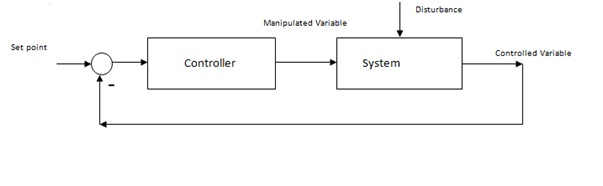
\includegraphics[scale = 20,width = 1\linewidth]{Vikas_self/report_tex/Closed Loop Circuit.jpg}
	\caption{Closed Loop Circuit}
\end{figure}

\begin{align}
V(s) = \frac {G_c(s) G(s)}{1+G_c(s) G(s)}
\end{align}

Where\\
V(s) : Overall closed-loop transfer function\\
$G_c$(s) : Controller transfer function\\
G(s) : System transfer function.\\ \\\\
Therefore,

\begin{align*}
G_c(s) = \frac 1{G(s)} \frac {V(s)}{1-V(s)}
\end{align*}
Let the desired closed loop transfer function be of form
\begin{align}
V(s)=\frac 1{(\tau_{cl}s+1)}\\
G(s)=\frac {K_p}{(\tau\_p s+1)}
\end{align}
By using the equations for G(s) and V(s), we get:

\begin{align}
G(c)=K_c(1 + \frac {1}{\tau s})
\end{align}

Where,\\
$K_c = \frac 1{K_p} (\tau_p / \tau_{cl} )$\\
$\tau_i = \tau_p$

\textit{When $K_p$ and $\tau_p$ are known as a function of time, the values of $K_c$ and $\tau_i$ can be found as function of temperature as well.}
\newpage
\section{Ziegler Nichols Tuning}
For the Ziegler Nichols Tuning, we use the step response of the open loop experiment.

\begin{figure}[h]
	\centering
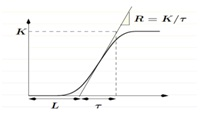
\includegraphics[width = 0.7\linewidth]{Vikas_self/report_tex/ziegler.jpg}
	\caption{Tangent Approach to Ziegler Nichols Tuning}
	\label{ziegler}
\end{figure}

%\begin{figure}[h]
%\centering
%	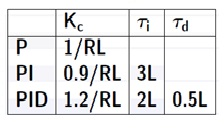
\includegraphics[scale = .5,width=0.50\linewidth]{pidziegler.jpg}
%	\label{fig:pidziegler}
%\end{figure}

\begin{table}[h]
	\centering
	\begin{tabular}{|l||c|c|c|}\hline
		  & $K_c$ & $\tau_i$ & $\tau_d$ \\ \hline \hline
		P & 1/RL & & \\ \hline
		PI & 0.9/RL & 3L& \\ \hline
		PID & 1.2/RL & 2L & .5L\\ \hline
	\end{tabular}
	\caption{Ziegler Nichols PID Settings}
	\label{ziegler}
\end{table}


Table \ref{ziegler} gives the PID settings. In this approach too, for every open step test, K and $\tau$ are found and correlated as function of average temperature and PID settings are then found as functions of temperature.
\\Note: For a First Order transfer function that we are assuming,
\begin{itemize}
	\item $K_p$ $\approx$ K 
	\item $\tau_p$ $\approx$ $\tau$
\end{itemize}

\section{Step Test Experiments and Parmeter Estimation}
Several Open Loop step test experiments were carried out and the values of the open loop parameters were found by curve fitting. The results are shown.
\subsection{Step Test Experiments}
\subsubsection{Step Change in Heater Reading from 10 to 15}

	
\begin{figure}
\centering	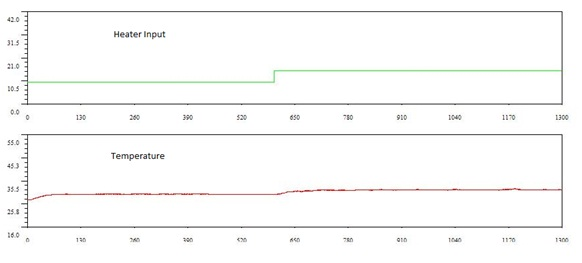
\includegraphics[width=0.7\textwidth]{Vikas_self/report_tex/parameter_estimation/10to15.jpg}
	\caption{Step Responce for Heater Reading 10 to 15}
	\label{fig:10to15}
\end{figure}

	
	
\begin{figure}[h]
\centering
	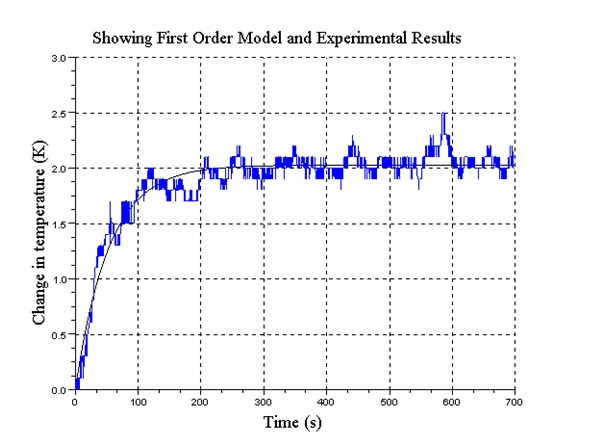
\includegraphics[width = .75\textwidth]{Vikas_self/report_tex/parameter_estimation/optimized10to15.jpg}
		\caption{Step Response for Heater reading 10 to 15 in terms of Deviation}
	\label{optimized10to15}
\end{figure}

\newpage
\subsubsection{Step Change in Heater Reading from 20 to 25}
\begin{figure}[h]
\centering
	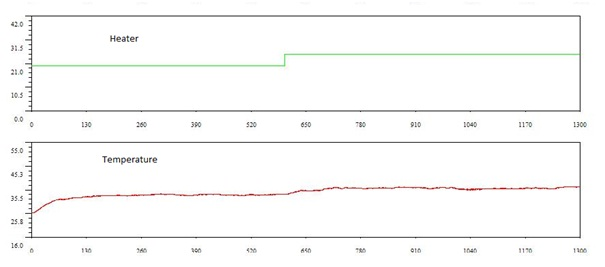
\includegraphics[width = 0.7\textwidth]{Vikas_self/report_tex/parameter_estimation/20to25.jpg}
		\caption{Step Responce for Heater Reading 20 to 25}
	\label{fig:20to25}
\end{figure}
%
\begin{figure}[h]
\centering
	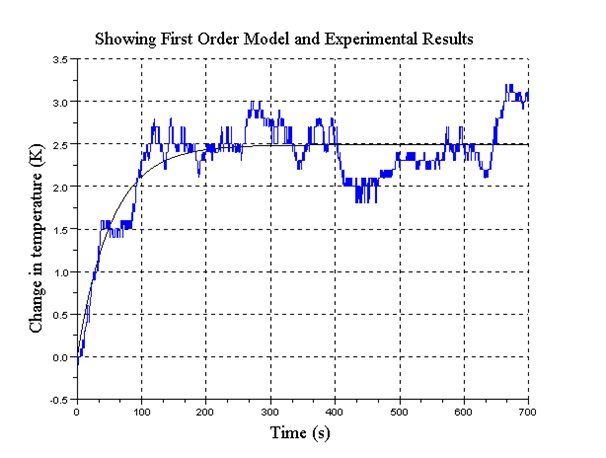
\includegraphics[width = .7\textwidth]{Vikas_self/report_tex/parameter_estimation/optimized20to25.jpg}
		\caption{Step Response for Heater reading 20 to 25 in terms of Deviation}
	\label{optimized20to25}
\end{figure}
\newpage
\subsubsection{Step Change in Heater Reading from 30 to 35}
%
\begin{figure}[h]
\centering
	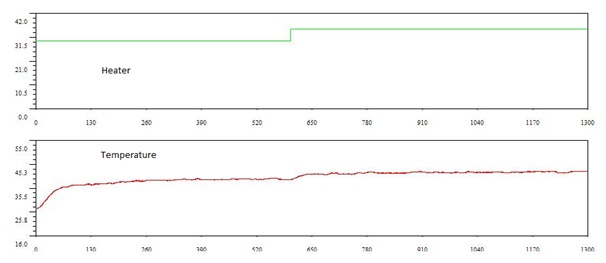
\includegraphics[width = 0.7\textwidth]{Vikas_self/report_tex/parameter_estimation/30to35.jpg}
		\caption{Step Responce for Heater Reading 30 to 35}
	\label{fig:30to35}
\end{figure}
%
\begin{figure}[h]
\centering
	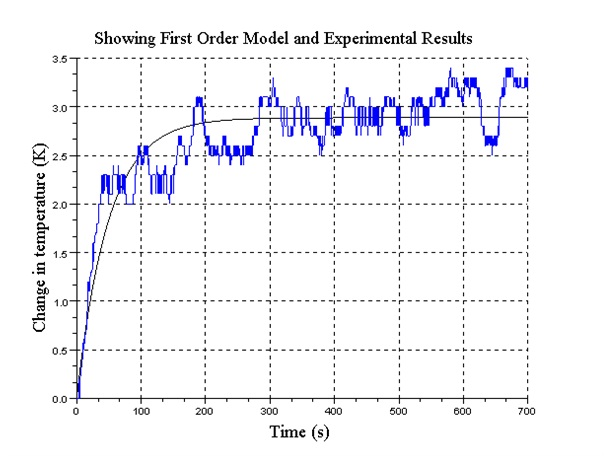
\includegraphics[width = .75\textwidth]{Vikas_self/report_tex/parameter_estimation/optimized30to35.jpg}
		\caption{Step Response for Heater reading 30 to 35 in terms of Deviation}
	\label{optimized30to35}
\end{figure}

\newpage
\subsubsection{The Open Loop Parameters}
\begin{table}[h]
	\begin{tabular}{|c|c|c|c|c|}\hline
	Initial Heater Reading&Final Heater Reading&Average Temperature($^0$C)&$K_p$&$\tau_p$\\ \hline \hline
	10	&15	&31.57	&0.41	&53.37\\ \hline
	20	&25	&36.00	&0.50	&52.64\\ \hline
	30	&35	&41.79	&0.58	&49.21\\ \hline
		
	\end{tabular}
	\caption{Open Loop Parameters}
	\label{tab:OpenLoopParameters}
\end{table}

It can be seen from the graphs that there is a lag of approximately 6 seconds in each experiment. 

\subsection{Conventional Controller Design}
\begin{enumerate}
	\item PI Controller using Ziegler Nichols Tuning with the results of the first step test experiment: 
\begin{itemize}
	\item Kc  = 19.75 
	\item $\tau_i$ = 18

\end{itemize}


	\item PID Controller using Ziegler Nichols Tuning with the results of the first step test experiment: 
\begin{itemize}
	\item Kc  = 26.327 
	\item $\tau_i$ = 12
	\item $\tau_d$ = 3

\end{itemize}


	\item PI Controller Using Direct Synthesis on the results of the second step test experiment ($\tau_{cl}$ is taken as $\tau_p$/2):
\begin{itemize}
	\item Kc  = 4.02
	\item $\tau_i$ = 52.645

\end{itemize}


\end{enumerate}
\subsection{Self Tuning Controller Design}
\label{selftuningdesign}
The graphs showing the variation of Kp and $\tau_p$ are shown below:

\begin{figure}[h]
\centering
	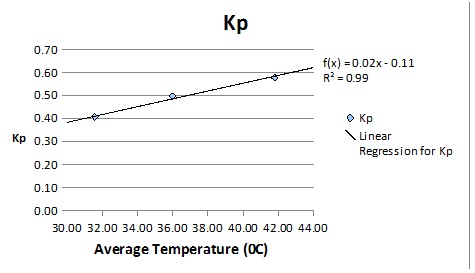
\includegraphics[width = \textwidth]{Vikas_self/report_tex/parameter_estimation/kp.jpg}
		\caption{Variation of $K_p$ with temperature}
	\label{kp}
\end{figure}

\begin{figure}
\centering
	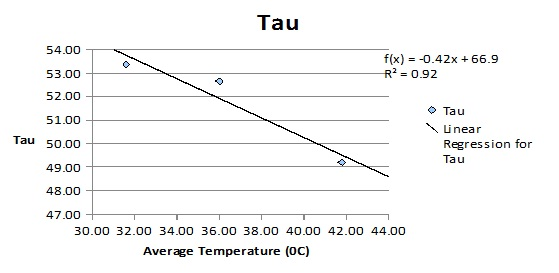
\includegraphics[width = \textwidth]{Vikas_self/report_tex/parameter_estimation/taup.jpg}
		\caption{Variation of $\tau_p$ with temperature}
	\label{taup}
\end{figure}
\newpage
\begin{enumerate}
	\item \textbf{PI Controller using Ziegler Nichols Tuning:} \\
	
	L = 6\\
	R = (0.016$\times$T-0.114)/(66.90-0.415$\times$T) where T is the temperature\\
	Kc = 0.9(66.90-0.415T)/6(0.016T-0.114) \\
		 = (60.21 - 0.3735T)/(0.096T - 0.684)\\
	% 0.9$\times$(66.90-0.415$\times$T)/6$\times$(0.016$\times$T-0.114)\\
	$\tau_i$ = 3 $\times$ 6 = 18\\

	\item \textbf{PID Controller using Ziegler Nichols Tuning:} \\
	
	L = 6\\
	R = (0.016 $\times$ T-0.114)/(66.90-0.415 $\times$ T) where T is the temperature\\
	K = 1.2(66.90-0.415T)/6(0.016T-0.114)\\
		= (80.28 - 0.498T)/(0.096T - 0.684)\\
	%1.2$\times$(66.90-0.415 $\times$ T)/6$\times$(0.016 $\times$ T-0.114)\\
	$\tau_i$ = 2 $\times$ 6 = 12\\
	$\tau_d$ = 0.5$\times$6 = 3\\

	\item \textbf{PI Controller using Direct Synthesis ($\tau_{cl}$ is taken as $\tau_p$/2):}\\

	K = 2/(0.016$\times$T-0.114)\\
	$\tau_i$ = (66.90-0.415$\times$T) where T is the temperature\\

\end{enumerate}


\section{Implementation}
\subsection{PI Controller}
\begin{figure}[h]
\centering
	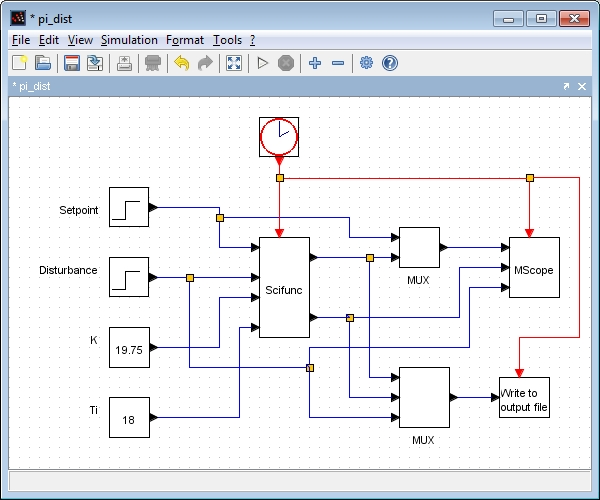
\includegraphics[ width =0.7\textwidth]{Vikas_self/report_tex/implementation/Pi_dist_xcos.jpg}
		\caption{Xcos Diagram for PI Controller}
	\label{PI}
\end{figure}

The PI Controller in Continuous Time is given by:
\begin{align*}
	u(t) = K \left[e(t) + \frac 1{\tau_i}\int_0^t e(t)dt\right]
\end{align*}
On taking Laplace Transform, we obtain:
\begin{align*}
	u(s) = K \left[1 + \frac 1{\tau_i s}\right]e(s)
\end{align*}
By mapping the above to discrete time interval using Backward Difference Approximation
\begin{align*}
	u(n) = K \left[1 + \frac{T_s}{\tau_i} \frac{z}{z-1}\right]e(n)
\end{align*}
On Cross Multiplication, we obtain:
\begin{align*}
	(z-1)\times u(n) = K \left[(z-1) + \frac{T_s}{\tau_i} (z)\right]e(n)
\end{align*}
We devide by z, and using the shifting theorem, we obtain:
\begin{align*}
	 u(n) - u(n-1) = K \left[e(n) - e(n-1) + \frac{T_s}{\tau_i} e(n)\right]
\end{align*}
The PI Controller is usually written as:
\begin{align}
	 u(n) = u(n-1) + s_0 e(n) + s_1 e(n-1)
\end{align}
Where,
\begin{align*}
s_0 &= K\left(1+ \frac{T_s}{\tau_i}\right)\\
s_1 &= -K
\end{align*}



\subsection{PID Controller}
\begin{figure}[h]
\centering
	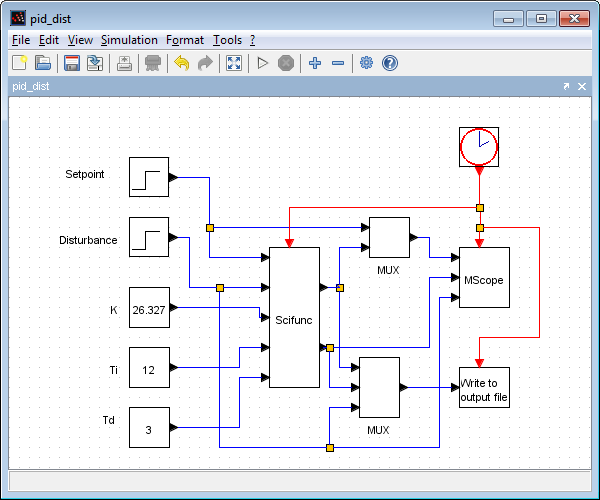
\includegraphics[width =0.7\textwidth]{Vikas_self/report_tex/implementation/pid_dist.png}
		\caption{Xcos Diagram for PID Controller}
	\label{PID}
\end{figure}

The PID Controller in Continuous Time is given by:
\begin{align*}
	u(t) = K \left[e(t) + \frac 1{\tau_i}\int_0^t e(t)dt + \tau_d \frac{de(t)}{dt}\right]
\end{align*}
On taking Laplace Transform, we obtain:
\begin{align*}
	u(s) = K \left[1 + \frac 1{\tau_i s} + \tau_d s\right]e(s)
\end{align*}
By mapping the above to discrete time interval by using the Trapezoidal Approximation for integral mode and Backward Difference Approximation for Derivative mode
\begin{align*}
	u(n) = K \left[1 + \frac{T_s}{\tau_i} \frac{z}{z-1} + \frac{\tau_d}{T_s} \frac{z-1}{z}\right]e(n)
\end{align*}
On Cross Multiplication, we obtain:
\begin{align*}
	(z^2-z)\times u(n) = K \left[(z^2-z) + \frac{T_s}{\tau_i} (z^2) + \frac{\tau_d}{T_s} (z-1)^2\right]e(n)
\end{align*}
We devide by z, and using the shifting theorem, we obtain:
\begin{align*}
	 u(n) - u(n-1) = K \left[e(n) - e(n-1) + \frac{T_s}{\tau_i} e(n) + \frac{\tau_d}{T_s}\left\{e(n) - 2e(n-1) + e(n-1)\right\}\right]
\end{align*}
The PID Controller is usually written as:
\begin{align}
	 u(n) = u(n-1) + s_0 e(n) + s_1 e(n-1) + s_2 e(n-2)
\end{align}
Where,
\begin{align*}
s_0 &= K\left(1+ \frac{T_s}{\tau_i} + \frac{\tau_d}{T_s}\right)\\
s_1 &= K\left[-1 - 2\frac{\tau_d}{T_s}\right]\\
s_2 &= K\left[\frac{\tau_d}{T_s}\right]
\end{align*}

\newpage
\subsection{Self Tuning Controller}
\begin{figure}[h]
\centering
	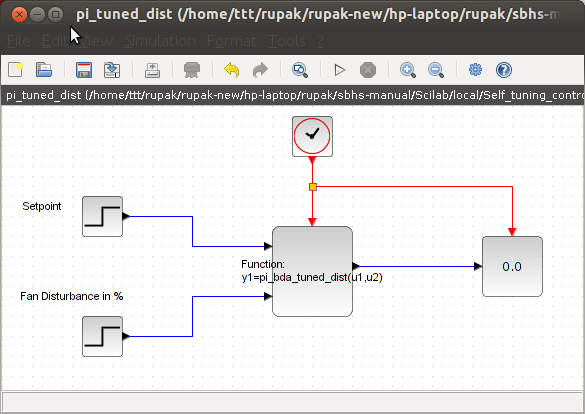
\includegraphics[width = \textwidth]{Vikas_self/report_tex/implementation/pi_dist_self.png}
		\caption{Xcos Diagram for Self Tuning Controller}
	\label{selftuning}
\end{figure}

The parameters of the Controller are determined dynamically using the temperature values during every sampling time. For this, the formulae derived in section \ref{selftuningdesign} are used. The formulae for the control effort are same as the conventional PI and PID controllers. So the PI/PID settings are calculated for every sampling time and the control effort is calculated thereafter using the formulae derived for conventional controllers.
%
%
%	
\section{Set Point Tracking}

The main aim of the controller is to track the set point and to reject disturbances. When the set point of the controlled variable (temperature in this case) is changed, the controller should work in such a manner that the actual temperature follows the set point as close as possible.\\

In this project, several experiments were conducted with the self tuning and conventional PI/PID Controllers. Table \ref{spt} shows the set point changes given during the various experiments that were conducted with conventional and self tuning controllers designed using several methods.
\begin{table}[h]
	\centering
		\begin{tabular}{||c|c|c|}\hline
			&Conventional Controller&Self Tuning Controller\\\hline \hline
		Direct Synthesis PI&32$^0$C to $37^0$C&32$^0$C to 37$^0$C\\
											 &35$^0$C to 45$^0$C&35$^0$C to 45$^0$C\\\hline
		Ziegler Nichols PI&32$^0$C to 37$^0$C&32$^0$C to 37$^0$C\\
												&35$^0$C to 45$^0$C&35$^0$C to 45$^0$C\\
												&40$^0$C to 45$^0$C&35$^0$C to 45$^0$C\\\hline
		Ziegler Nichols PID&31$^0$C to 45$^0$C&32$^0$C to 46$^0$C\\
												&32$^0$C to 37$^0$C&32$^0$C to 37$^0$C\\\hline
		\end{tabular}
	\caption{Set Point Changes in experiments conducted for Set Point Tracking}
	\label{spt}
\end{table}
\newpage
\subsection{PI Controller designed by Direct Synthesis}
The results of the experiments carried out for the self tuning PI controller using direct synthesis method are shown. The upper plot shows the variations of the set point temperature (the black line) and the actual temperature (the green line) in the SBHS. The lower plot shows the control effort.
\begin{figure}[h]
	\centering
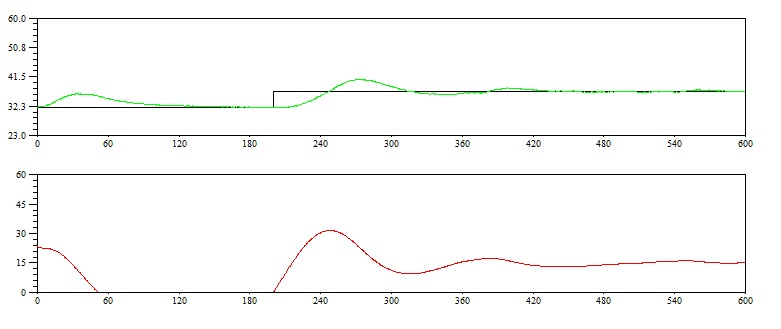
\includegraphics[width=0.7\textwidth]{Vikas_self/report_tex/PID_results/self_tuning/NewSetpoint_change/DirectSynthesis/step32to37.jpg}
	\caption{Result for Self Tuning Controller designed using Direct Synthesis for Set Point going from 32$^0$C to 37$^0$C}
	\label{fig:step32to37}
\end{figure}

Although there is a small overshoot, the controller is able to make the actual temperature follow the set point temperature quiet closely. Looking at higher values of set point changes, the result for set point change going from 35$^0$C to 45$^0$C is shown.
\begin{figure}[h]
	\centering
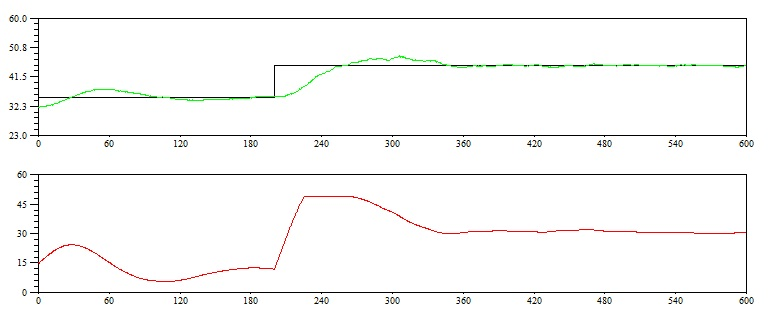
\includegraphics[width=0.7\textwidth]{Vikas_self/report_tex/PID_results/self_tuning/NewSetpoint_change/DirectSynthesis/step35to45.jpg}
	\caption{Result for Self Tuning Controller designed using Direct Synthesis for Set Point going from 35$^0$C to 45$^0$C }
	\label{fig:step35to45}
\end{figure}

For a higher set point change also, the controller is able to make the temperature follow the set point closely. Notice the abrupt change in the control effort as soon as the step change in the set point is encountered.\\For comparison, results of experiments done with conventional PI controller designed using the Direct Synthesis method are also shown.

\begin{figure}[h]
	\centering
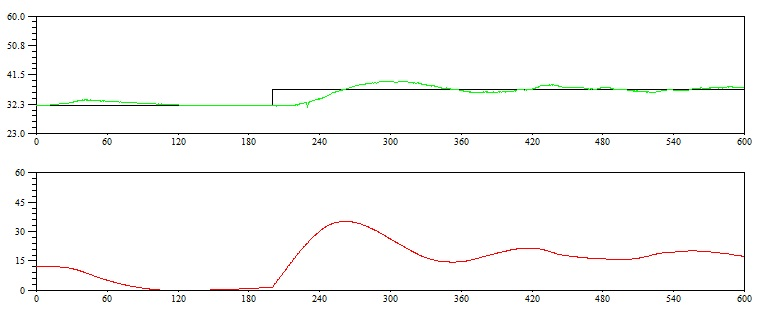
\includegraphics[width=0.7\textwidth]{Vikas_self/report_tex/PID_results/Conventional_Tuning/Setpointchange/Direct_Synthesis/step32to37.jpg}
	\caption{Result for Conventional Controller designed using Direct Synthesis for Set Point going from 32$^0$C to 37$^0$C }
	%\label{fig:step32to37}
\end{figure}

\begin{figure}[h]
	\centering
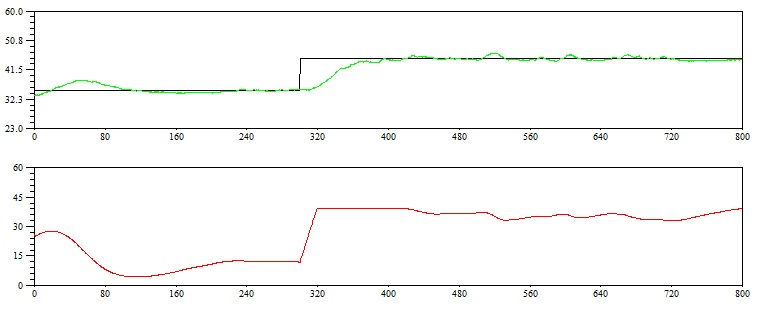
\includegraphics[width=.7\textwidth]{Vikas_self/report_tex/PID_results/Conventional_Tuning/Setpointchange/Direct_Synthesis/step35to45.jpg}
	\caption{Result for Conventional Controller designed using Direct Synthesis for Set Point going from 35$^0$C to 45$^0$C }
\end{figure}
As can been seen from the graph, the self tuning controller stabilised the temperature faster.
\newpage


%PI ZN
\subsection{PI Controller using Ziegler Nichols Tuning}
The results of the of the experiments carried out for the self tuning PI controller using Ziegler Nichols tuning method are shown. The upper plot shows the variations of the set point temperature (the black line) and the actual temperature (the green line) in the SBHS. The lower plot shows the control effort.
\begin{figure}[h]
	
		\centering
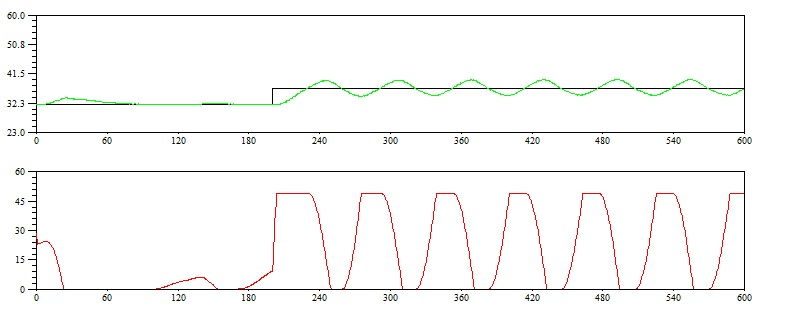
\includegraphics[width=0.7\textwidth]{Vikas_self/report_tex/PID_results/self_tuning/NewSetpoint_change/PI/step32to37.jpg}
		\caption{Result for Self Tuning Controller designed using Ziegler Nichols Tuning for Set Point going from 32$^0$C to 37$^0$C}
\end{figure}

Although there are oscillations, the temperature remains near the set point. The result for a higher value of set point change is also shown.
\begin{figure}[h]
	\centering
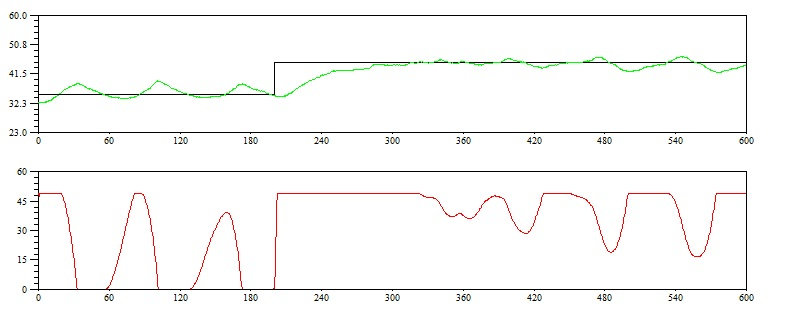
\includegraphics[width=0.7\textwidth]{Vikas_self/report_tex/PID_results/self_tuning/NewSetpoint_change/PI/step35to45.jpg}
		\caption{Result for Self Tuning Controller designed using Ziegler Nichols Tuning for Set Point going from 35$^0$C to 45$^0$C}

	
\end{figure}

For this experiment, the controller is able to make the temperature follow the set point closely. The fluctuations may be due to noises and the surrounding conditions.The plot for result of an experiment with another value of set point change is also shown.

\begin{figure}[h]
\centering
	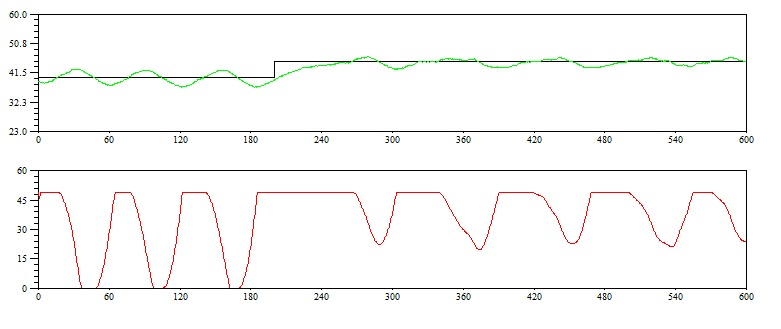
\includegraphics[ width=0.7\textwidth]{Vikas_self/report_tex/PID_results/self_tuning/NewSetpoint_change/PI/step40to45.jpg}
		\caption{Result for Self Tuning Controller designed using Ziegler Nichols Tuning for Set Point going from 40$^0$C to 45$^0$C}
\end{figure}
In this experiment too, the controller is able to keep the temperature close to the set point and it stabilises fast.\\
For comparison, results of experiments done with conventional PI controller designed using the Ziegler Nichols method are also shown.

\begin{figure}[h]
	\centering	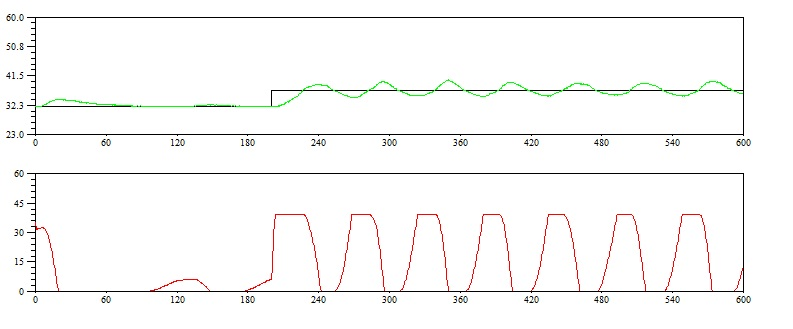
\includegraphics[width=0.7\textwidth]{Vikas_self/report_tex/PID_results/Conventional_Tuning/Setpointchange/PI/step32to37.jpg}
	\caption{Result for Conventional Controller designed using Ziegler Nichols Tuning for Set Point going from 32$^0$C to 37$^0$C }
\end{figure}
\newpage
\begin{figure}[h]
	\centering	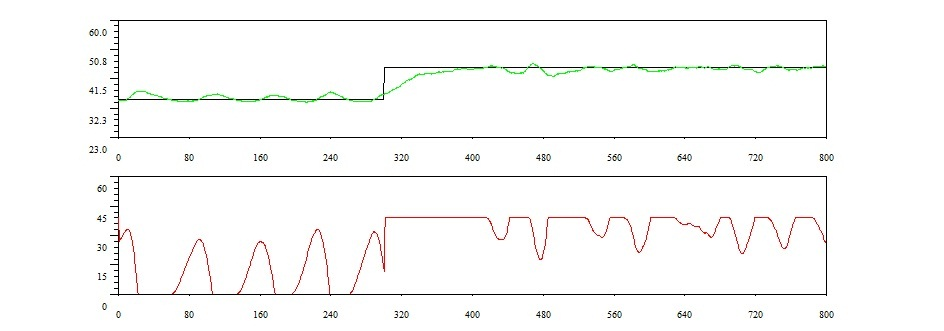
\includegraphics[width=0.7\textwidth]{Vikas_self/report_tex/PID_results/Conventional_Tuning/Setpointchange/PI/step35to45.jpg}
	\caption{Result for Conventional Controller designed using Ziegler Nichols Tuning for Set Point going from 35$^0$C to 45$^0$C }
\end{figure}

\begin{figure}[h]
		\centering
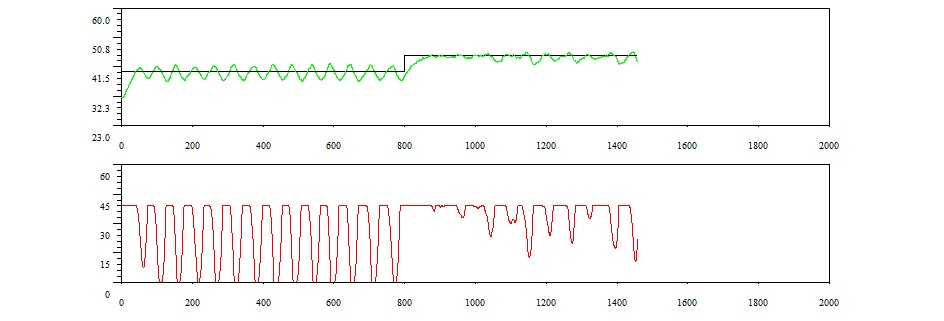
\includegraphics[width=0.7\textwidth]{Vikas_self/report_tex/PID_results/Conventional_Tuning/Setpointchange/PI/step40to45.jpg}
	\caption{Result for Conventional Controller designed using Ziegler Nichols Tuning for Set Point going from 40$^0$C to 45$^0$C }
\end{figure}

For set point change from 40$^0$C to 45$^0$C, the self tuning controller showed small oscillations, but the conventional controller shows bigger oscillations.
\newpage


%pid zn
\subsection{PID Controller using Ziegler Nichols Tuning}\label{pidzn}
The results of the of the experiments carried out for the self tuning PID controller using Ziegler Nichols tuning method are shown. The upper plot shows the variations of the set point temperature (the black line) and the actual temperature (the purple line) in the SBHS. The lower plot shows the control effort.

\begin{figure}[h]
	\centering
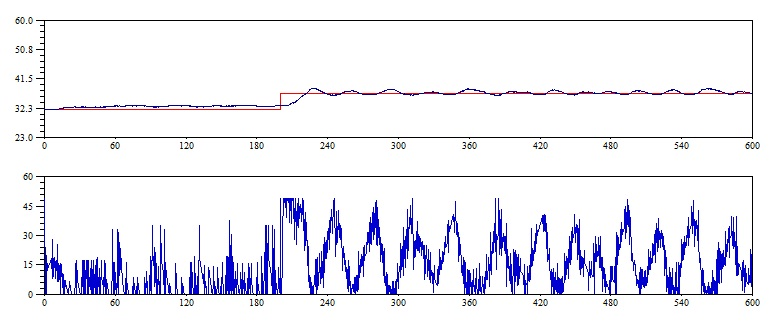
\includegraphics[width=0.7\textwidth]{Vikas_self/report_tex/PID_results/self_tuning/NewSetpoint_change/PID/step32to37.jpg}
	\caption{Result for Self Tuning PID Controller designed using Ziegler Nichols Tuning for Set Point going from 32$^0$C to 37$^0$C}
\end{figure}


\begin{figure}[h]
	\centering
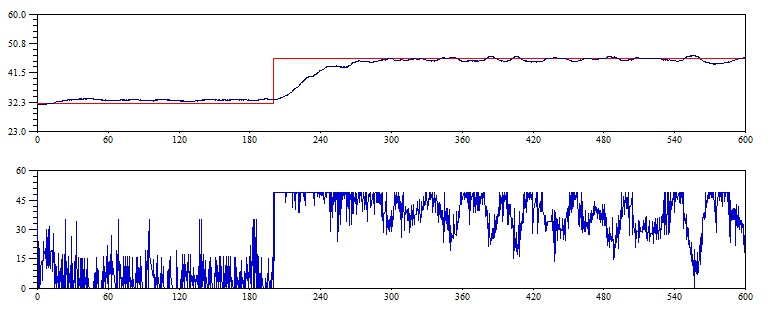
\includegraphics[width=0.7\textwidth]{Vikas_self/report_tex/PID_results/self_tuning/NewSetpoint_change/PID/step32to46.jpg}
	\caption{Result for Self Tuning PID Controller designed using Ziegler Nichols Tuning for Set Point going from 32$^0$C to 46$^0$C}
\end{figure}

From the graph it can be seen that for both the above experiments, the self tuning PID controller is able to keep the temperature close to the set point and the stabilisation is also fast. For comparison, plots for experiments conducted with conventional PID controller designed using Ziegler Nichols method are also shown.

\begin{figure}[h]
	\centering
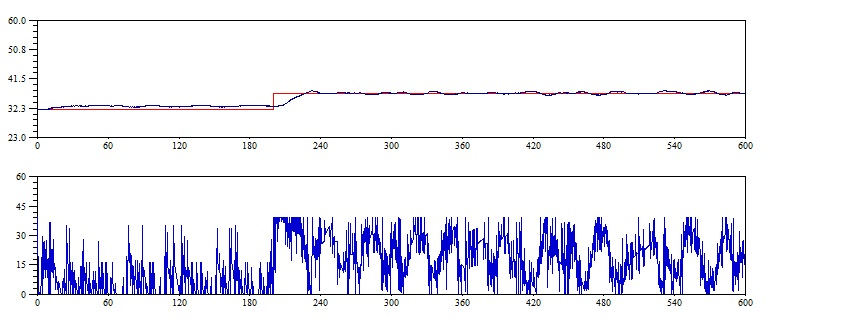
\includegraphics[width=0.7\textwidth]{Vikas_self/report_tex/PID_results/Conventional_Tuning/Setpointchange/PID/step32to37.jpg}
	\caption{Result for Conventional PID Controller designed using Ziegler Nichols Tuning for Set Point going from 32$^0$C to 37$^0$C }
	\label{fig:step31to45}
\end{figure}


\begin{figure}[h]
	\centering
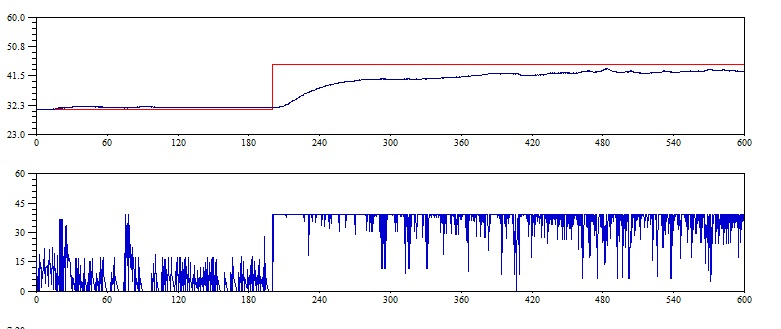
\includegraphics[width=0.7\textwidth]{Vikas_self/report_tex/PID_results/Conventional_Tuning/Setpointchange/PID/step31to45.jpg}
	\caption{Result for Conventional PID Controller designed using Ziegler Nichols Tuning for Set Point going from 31$^0$C to 45$^0$C }
	\label{fig:step31to45}
\end{figure}

From the above graph we can see that the conventional PID controller is not able to make the temperature close to the set point when the set point value is 45$^0$C. The self tuning PID controller had successfully brought the temperature to 45$^0$C.

\subsection{Conclusion}
The self tuning PI controller is able to accomplish the aim of keeping the temperature as close as possible to the set point. Although it may show some initial overshoot or oscillation for some values of set point change, the time needed for stabilisation is low. There may also some cases where the conventional controller shows bigger oscillations than the self tuning controller.\\

The PI controllers, both conventional and self tuning, show oscillations for some values of set point change. To eliminate the oscillations, when we use the PID Controller, the self tuning design definately seems to be a better option because for higher values of set point change, the self tuning PID controller shows a better performance than the conventional controller as seen in section \ref{pidzn}.

\section{Disturbance Rejection}

Apart from tracking the set point, the system should also be able to reject disturbances. There may be several factors influencing the controlled variable and not all of them can be manipulated. Therefore, it becomes necessary for the controller not to let the changes in the non-manipulated vraibles to affect the controlled variable. This is called Disturbance Rejection.\\

In this system, the disturbance variable is the fan input. Therefore, the controller has to work in such a way that changes in the fan input doesn't affect the temperature in the SBHS.\\

In this project, several experiments were conducted with the self tuning and conventional PI/PID Controllers. Table \ref{dist} shows the fan input changes given during the various experiments that were conducted with conventional and self tuning controllers designed using several methods.\\
\begin{table}[h]
	\centering
		\begin{tabular}{||c|c|c|}\hline
			&Conventional Controller&Self Tuning Controller\\\hline \hline
		Direct Synthesis PI&50 to 100&50 to 100\\
											 &100 to 50&100 to 50\\\hline
		Ziegler Nichols PI &50 to 100&50 to 100\\
												&100 to 50&100 to 50 \\\hline
		Ziegler Nichols PID&50 to 100&50 to 100\\
												&100 to 50&100 to 50\\\hline
		\end{tabular}
	\caption{Fan Input Changes in experiments conducted for Disturbance Rejection}
	\label{dist}
\end{table}


\subsection{PI Controller designed by Direct Synthesis}
The results of the experiments carried out for the self tuning PI controller using direct synthesis method are shown. The upper plot shows the variations of the set point temperature (the black line) and the actual temperature (the green line) in the SBHS. The second plot shows the control effort and the third shows the fan input.

\begin{figure}[h]
	\centering
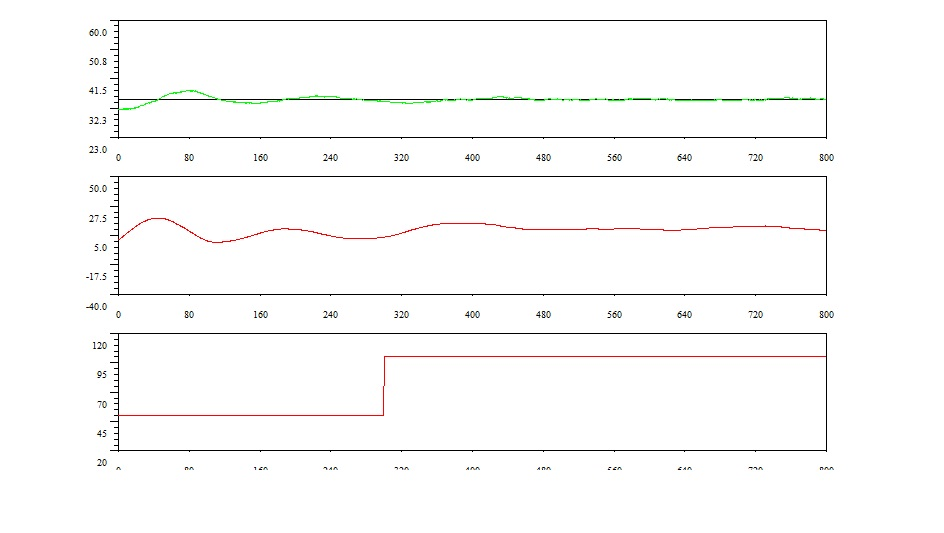
\includegraphics[width=0.7\linewidth]{Vikas_self/report_tex/PID_results/self_tuning/FanDisturbance/DirectSynthesis/step50to100.jpg}
	\caption{Results for Fan Input Change from 50 to 100 for Self Tuning PI Controller  designed using Direct Synthesis}
\end{figure}
The change in the fan input introduces a small dent in the temperature. However, the controller brings the temperature back to the set point. Notice the slight change in the controller behaviour on encountering the fan input change. The time taken for stabilising back is also low.
\newpage
Here, results for fan input change from 100 to 50 are also shown.
\begin{figure}[h]
	\centering
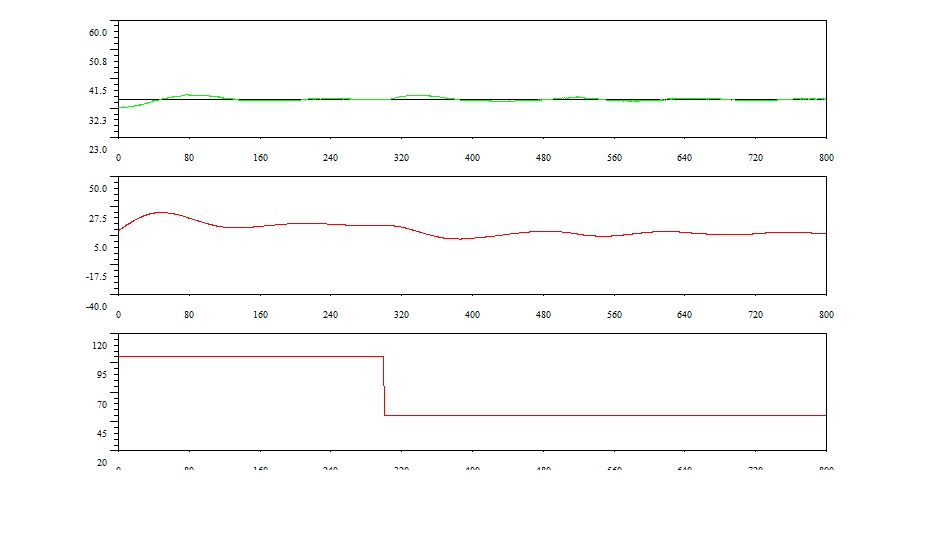
\includegraphics[width=0.7\linewidth]{Vikas_self/report_tex/PID_results/self_tuning/FanDisturbance/DirectSynthesis/step100to50.jpg}
	\caption{Results for Fan Input Change from 100 to 50 for Self Tuning PI Controller  designed using Direct Synthesis}
\end{figure}

In this figure also, the temperature clearly increses a bit when the step change in the fan input is encountered. However, it quickly stabilises back and continues to be close to the set point.\\

From the above two results, it is clear that the self tuning controller designed with direct syntheis has successfully rejected the disturbance.\\

For comparison, results of the disturbance change for conventional PI Controller designed with direct synthesis are also shown.
\newpage
\begin{figure}[h]
	\centering
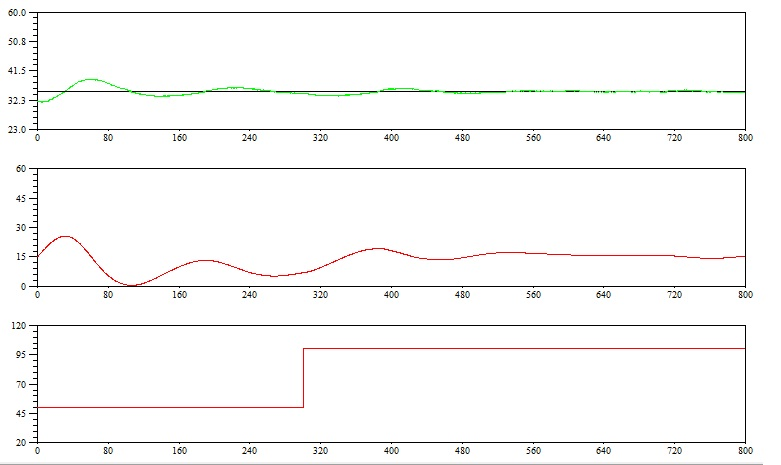
\includegraphics[width=.7\linewidth]{Vikas_self/report_tex/PID_results/Conventional_Tuning/Fan_disturbance/Direct_Systhesis/step50to100.jpg}
	\caption{Results for the Fan input change from 50 to 100 to Conventional PI Controller designed using Direct Synthesis}
\end{figure}

\begin{figure}[h]
	\centering
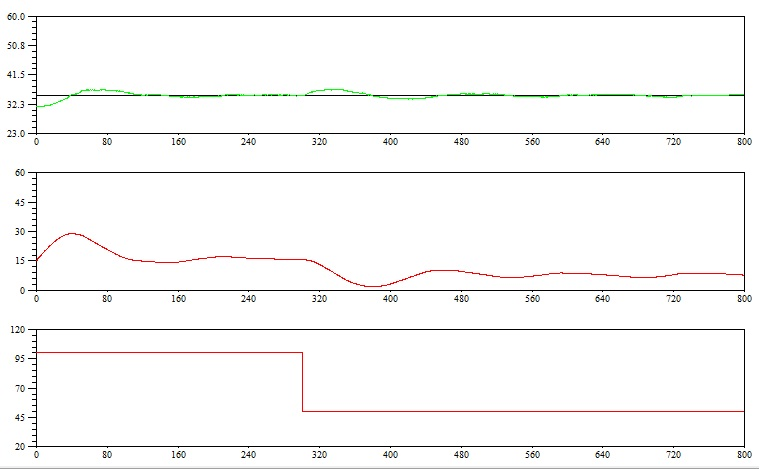
\includegraphics[width=.7\linewidth]{Vikas_self/report_tex/PID_results/Conventional_Tuning/Fan_disturbance/Direct_Systhesis/step100to50.jpg}
	\caption{Results for the Fan input change from 100 to 50 to Conventional PI Controller designed using Direct Synthesis}
\end{figure}

%pi zn
\newpage
\subsection{PI Controller using Ziegler Nichols Tuning}
The results of the experiments carried out for the self tuning PI controller using Ziegler Nichols method are shown. The upper plot shows the variations of the set point temperature (the black line) and the actual temperature (the green line) in the SBHS. The second plot shows the control effort and the third shows the fan input.
\begin{figure}[h]
	\centering
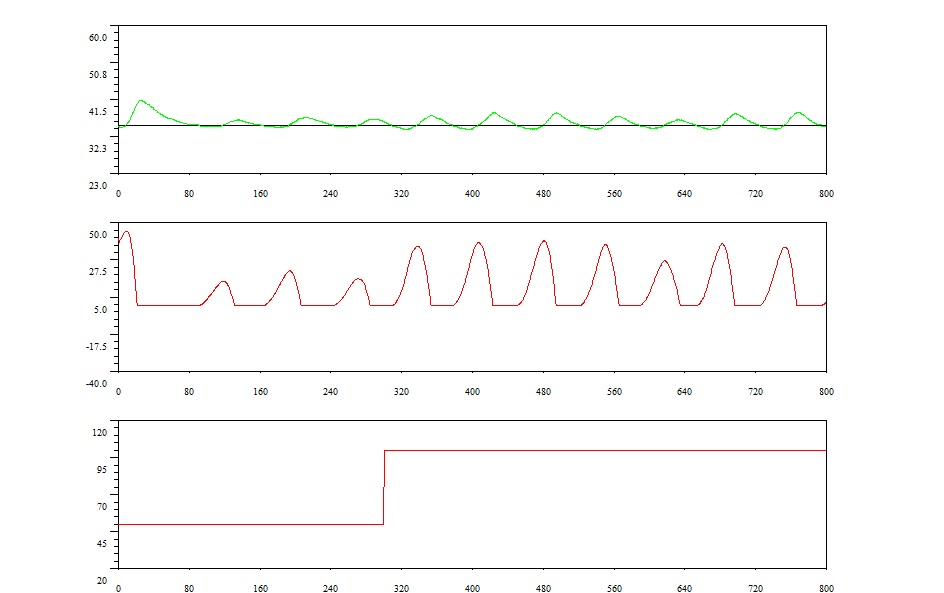
\includegraphics[width=0.7\textwidth]{Vikas_self/report_tex/PID_results/self_tuning/FanDisturbance/PI/step50to100final.jpg}
	
\caption{Results for Fan Input change from 50 to 100 given to Self Tuning PI Controller designed using Ziegler Nichols Method}
\end{figure}

Even on encountering the fan input change, the temperature remains close to the set point. Notice the change in the controller behaviour on encountering the fan input change. 
\newpage
Here, result for the fan input going from 100 to 50 is also shown.
\begin{figure}[h]
	\centering
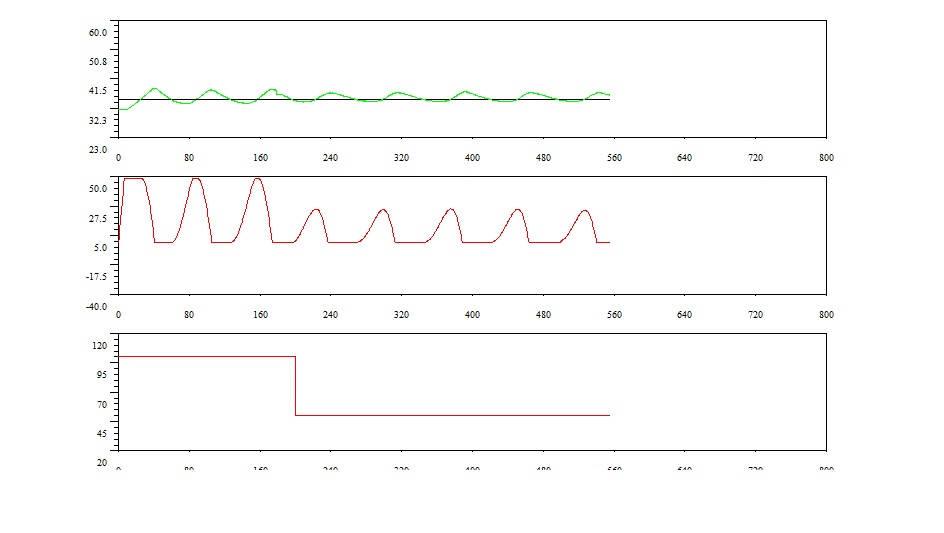
\includegraphics[width=0.7\textwidth]{Vikas_self/report_tex/PID_results/self_tuning/FanDisturbance/PI/step100to50.jpg}
	
\caption{Results for Fan Input change from 100 to 50 given to Self Tuning PI Controller designed using Ziegler Nichols Method}
\end{figure}

Here, a change in the control effort can be noticed. This change has been brought by the PI Controller to keept the temperature close to the set point.\\
From the above two results, it is clear that the self tuning controller designed with direct syntheis has successfully rejected the disturbance.\\
\newpage
For comparison, correspoding results are also shown for Conventional PI Controllers designed using ziegler nichols tuning.

\begin{figure}[h]
	\centering
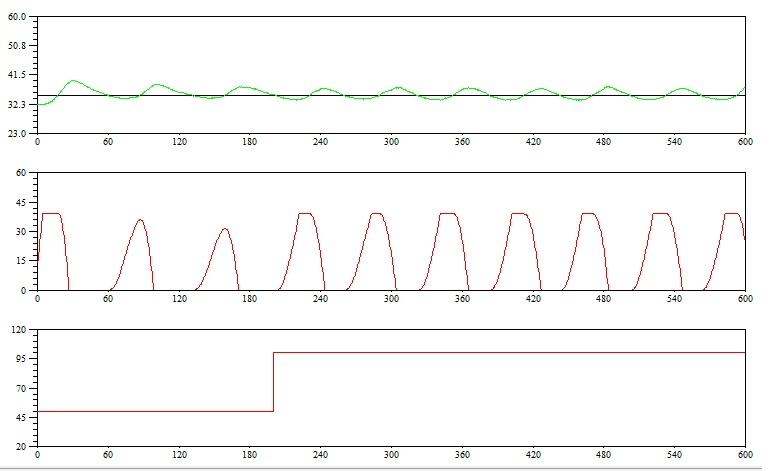
\includegraphics[width=.75\linewidth]{Vikas_self/report_tex/PID_results/Conventional_Tuning/Fan_disturbance/PI/step50to100.jpg}
	\caption{Results for the Fan input change from 50 to 100 to Conventional PI Controller designed using Ziegler Nichols Tuning}
\end{figure}

\begin{figure}[h]
	\centering
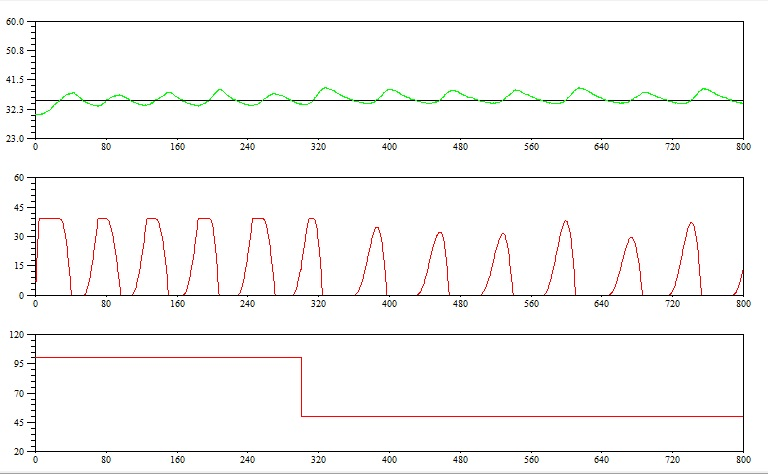
\includegraphics[width=.75\linewidth]{Vikas_self/report_tex/PID_results/Conventional_Tuning/Fan_disturbance/PI/step100to50.jpg}
	\caption{Results for the Fan input change from 100 to 50 to Conventional PI Controller designed using Ziegler Nichols Tuning}
\end{figure}


\newpage
\subsection{PID Controller using Ziegler Nichols Tuning}
The results of the experiments carried out for the self tuning PID controller using Ziegler Nichols method are shown. The upper plot shows the variations of the set point temperature (the black line) and the actual temperature (the purple line) in the SBHS. The second plot shows the control effort and the third shows the fan input.

\begin{figure}[h]
	\centering
		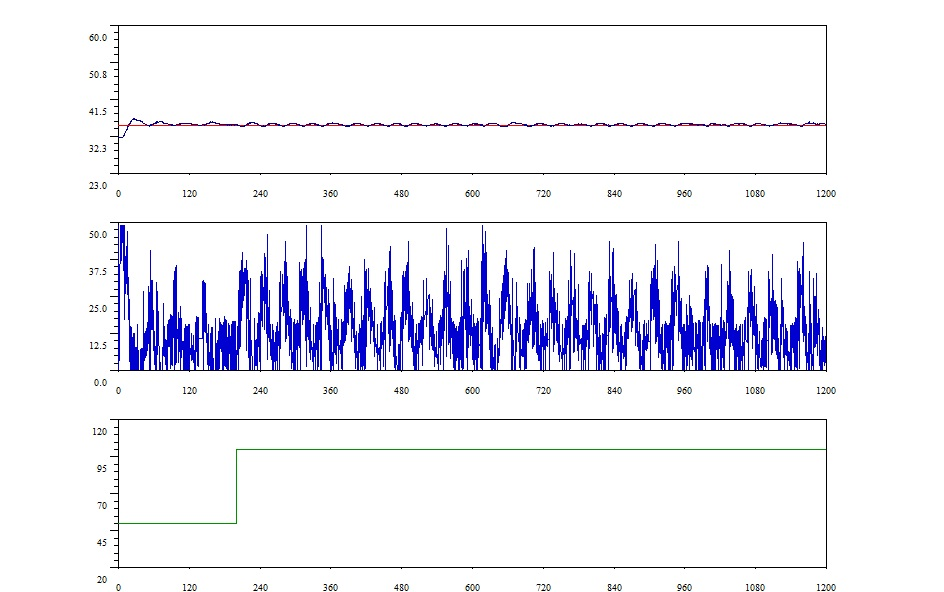
\includegraphics[width=0.7\linewidth]{Vikas_self/report_tex/PID_results/self_tuning/FanDisturbance/PID/step50to100.jpg}
\caption{Results for Fan Input change from 50 to 100 given to Self Tuning PID Controller designed using Ziegler Nichols Method}

\end{figure}

In this system also, on encountering the fan input change, the temperature remains close to the set point. Notice the change in the control effort profile when the change in the fan input is given.
\newpage
Here, result for the fan input going from 100 to 50 is also shown.
\begin{figure}[h]
	\centering
		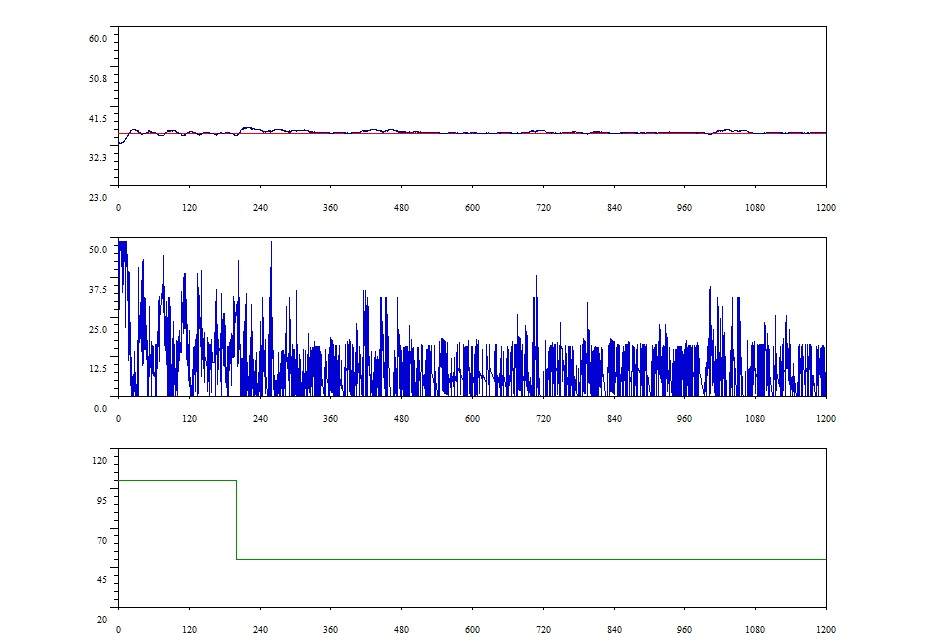
\includegraphics[ width=0.7\linewidth]{Vikas_self/report_tex/PID_results/self_tuning/FanDisturbance/PID/step100to50.jpg}
\caption{Results for Fan Input change from 100 to 50 given to Self Tuning PID Controller designed using Ziegler Nichols Method}

\end{figure}

In this figure also, the temperature clearly increses a bit when the step change in the fan input is encountered. However, it quickly stabilises back and continues to be close to the set point.
\newpage
For comparison, correspoding results are also shown for Conventional PID Controllers designed using ziegler nichols tuning.
\begin{figure}[h]
	\centering
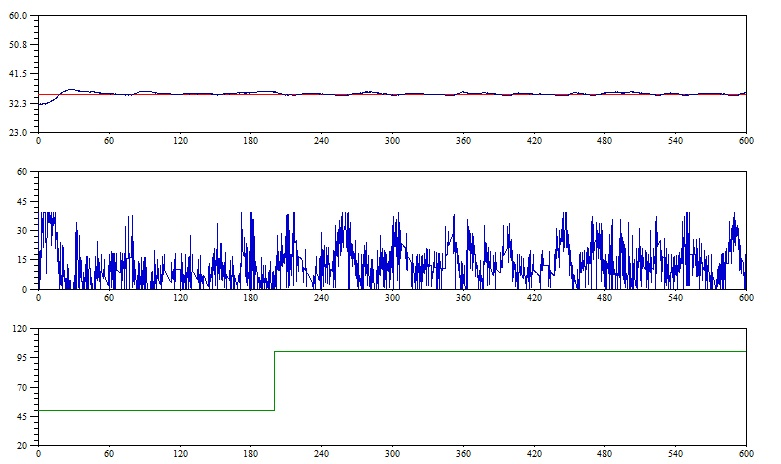
\includegraphics[width=.75\linewidth]{Vikas_self/report_tex/PID_results/Conventional_Tuning/Fan_disturbance/PID/step50to100.jpg}
	\caption{Results for the Fan input change from 50 to 100 to Conventional PID Controller designed using Ziegler Nichols Tuning}
	
\end{figure}

\begin{figure}[h]
	\centering
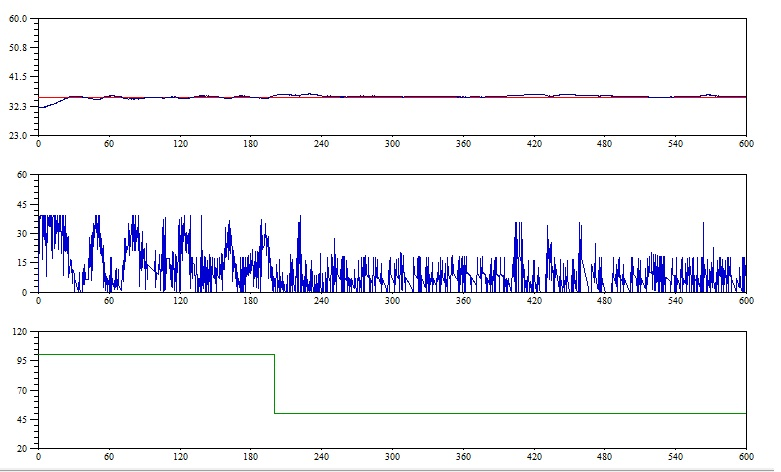
\includegraphics[width=.75\linewidth]{Vikas_self/report_tex/PID_results/Conventional_Tuning/Fan_disturbance/PID/step100to50.jpg}
	\caption{Results for the Fan input change from 100 to 50 to Conventional PID Controller designed using Ziegler Nichols Tuning}
	
\end{figure}

\subsection{Conclusion}
We see that the self tuning controller manages to keep the temperature close to the set point temperature, even when the change in fan input is encountered. This shows that it can reject the disturbances quite nicely.



\section{Implementing Self Tuning controller on SBHS, virtually}
The step by step procedure for conducting an experiment virtually is explained in section \ref{vlabsexpt}. The required .sce file is {\tt pi\_bda\_tuned\_dist\_virtual.sce} for example if you want to run the {\tt PI Controller Fan disturbance} experiment.  Under the {\tt virtual} folder there are two folders {\tt Self\_tuning\_controller} and {\tt SelfTuning\_Vikas}. You will find this file in the {\tt PIControllerFandisturbance} directory. The necessary code is listed in the section \ref{convcode_virtual} and \ref{selfcode_virtual}


\subsection{Serial Communication}
\begin{code}
  \ccaption{ser\_init.sce}{\ttfamily ser\_init.sce}
\lstinputlisting{Vikas_self/ser_init.sce}
\end{code}


\subsection{Conventional Controller, local}\label{convcode_local}
\subsection{Fan Disturbance in PI Controller}
\begin{code}
  \ccaption{pi\_bda\_dist.sci}{\ttfamily pi\_bda\_dist.sci}
\lstinputlisting{Scilab/local/Self_tuning_controller/ConventionalTuning_Vikas/PIControllerFandisturbance/pi_bda_dist.sci}
\end{code}


\subsubsection{Set Point Change in PI Controller}
\begin{code}
  \ccaption{pi\_bda.sci}{\ttfamily pi\_bda.sci}
\lstinputlisting{Scilab/local/Self_tuning_controller/ConventionalTuning_Vikas/PIControllersetpointchange/pi_bda.sci}
\end{code}



\subsubsection{Fan Disturbance to PID Controller}
\begin{code}
  \ccaption{pid\_bda\_dist.sci}{\ttfamily pid\_bda\_dist.sci}
\lstinputlisting{Scilab/local/Self_tuning_controller/ConventionalTuning_Vikas/PIDControllerFandisturbance/pid_bda_dist.sci}
\end{code}


\subsubsection{Set Point Change in PID Controller}
\begin{code}
  \ccaption{pid\_bda.sci}{\ttfamily pid\_bda.sci}
\lstinputlisting{Scilab/local/Self_tuning_controller/ConventionalTuning_Vikas/PIDControllersetpointchange/pid_bda.sci}
\end{code}



\subsection{Self Tuning Controller, local}\label{selfcode_local}
\subsubsection{Fan Discturbance to PI Controller}
\begin{code}
  \ccaption{pi\_bda\_tuned\_dist.sci}{\ttfamily pi\_bda\_tuned\_dist.sci}
\lstinputlisting{Scilab/local/Self_tuning_controller/SelfTuning_Vikas/PIControllerFandisturbance/pi_bda_tuned_dist.sci}
\end{code}


\subsubsection{Set Point Change to PI Controller}
\begin{code}
  \ccaption{pi\_bda\_tuned.sci}{\ttfamily pi\_bda\_tuned.sci}
\lstinputlisting{Scilab/local/Self_tuning_controller/SelfTuning_Vikas/PIControllersetpointchange/pi_bda_tuned.sci}
\end{code}

\subsubsection{Fan Disturbance to PID Controller}
\begin{code}
  \ccaption{pid\_bda\_tuned\_dist.sci}{\ttfamily pid\_bda\_tuned\_dist.sci}
\lstinputlisting{Scilab/local/Self_tuning_controller/SelfTuning_Vikas/PIDControllerFandisturbance/pid_bda_tuned_dist.sci}
\end{code}

\subsubsection{Set Point Change to PID Controller}
\begin{code}
  \ccaption{pid\_bda\_tuned.sci}{\ttfamily pid\_bda\_tuned.sci}
\lstinputlisting{Scilab/local/Self_tuning_controller/SelfTuning_Vikas/PIDControllersetpointchange/pid_bda_tuned.sci}
\end{code}






\subsection{Conventional Controller, virtual}\label{convcode_virtual}
\subsection{Fan Disturbance in PI Controller}
\begin{code}
  \ccaption{pi\_bda\_dist.sci}{\ttfamily pi\_bda\_dist.sci}
\lstinputlisting{Scilab/virtual/Self_tuning_controller/ConventionalTuning_Vikas/PIControllerFandisturbance/pi_bda_dist_virtual.sci}
\end{code}


\subsubsection{Set Point Change in PI Controller}
\begin{code}
  \ccaption{pi\_bda.sci}{\ttfamily pi\_bda.sci}
\lstinputlisting{Scilab/virtual/Self_tuning_controller/ConventionalTuning_Vikas/PIControllersetpointchange/pi_bda_virtual.sci}
\end{code}



\subsubsection{Fan Disturbance to PID Controller}
\begin{code}
  \ccaption{pid\_bda\_dist.sci}{\ttfamily pid\_bda\_dist.sci}
\lstinputlisting{Scilab/virtual/Self_tuning_controller/ConventionalTuning_Vikas/PIDControllerFandisturbance/pid_bda_dist_virtual.sci}
\end{code}


\subsubsection{Set Point Change in PID Controller}
\begin{code}
  \ccaption{pid\_bda.sci}{\ttfamily pid\_bda.sci}
\lstinputlisting{Scilab/virtual/Self_tuning_controller/ConventionalTuning_Vikas/PIDControllersetpointchange/pid_bda_virtual.sci}
\end{code}



\subsection{Self Tuning Controller, local}\label{selfcode_virtual}
\subsubsection{Fan Discturbance to PI Controller}
\begin{code}
  \ccaption{pi\_bda\_tuned\_dist.sci}{\ttfamily pi\_bda\_tuned\_dist.sci}
\lstinputlisting{Scilab/virtual/Self_tuning_controller/SelfTuning_Vikas/PIControllerFandisturbance/pi_bda_tuned_dist_virtual.sci}
\end{code}


\subsubsection{Set Point Change to PI Controller}
\begin{code}
  \ccaption{pi\_bda\_tuned.sci}{\ttfamily pi\_bda\_tuned.sci}
\lstinputlisting{Scilab/virtual/Self_tuning_controller/SelfTuning_Vikas/PIControllersetpointchange/pi_bda_tuned_virtual.sci}
\end{code}

\subsubsection{Fan Disturbance to PID Controller}
\begin{code}
  \ccaption{pid\_bda\_tuned\_dist.sci}{\ttfamily pid\_bda\_tuned\_dist.sci}
\lstinputlisting{Scilab/virtual/Self_tuning_controller/SelfTuning_Vikas/PIDControllerFandisturbance/pid_bda_tuned_dist_virtual.sci}
\end{code}

\subsubsection{Set Point Change to PID Controller}
\begin{code}
  \ccaption{pid\_bda\_tuned.sci}{\ttfamily pid\_bda\_tuned.sci}
\lstinputlisting{Scilab/virtual/Self_tuning_controller/SelfTuning_Vikas/PIDControllersetpointchange/pid_bda_tuned_virtual.sci}
\end{code}





%% <== End of hints
%%%%%%%%%%%%%%%%%%%%%%%%%%%%%%%%%%%%%%%%%%%%%%%%%%%%%%%%%%%%%



%%%%%%%%%%%%%%%%%%%%%%%%%%%%%%%%%%%%%%%%%%%%%%%%%%%%%%%%%%%%%
%% BIBLIOGRAPHY AND OTHER LISTS
%%%%%%%%%%%%%%%%%%%%%%%%%%%%%%%%%%%%%%%%%%%%%%%%%%%%%%%%%%%%%
%% A small distance to the other stuff in the table of contents (toc)
%\addtocontents{toc}{\protect\vspace*{\baselineskip}}



%% The Bibliography
%% ==> You need a file 'literature.bib' for this.
%% ==> You need to run BibTeX for this (Project | Properties... | Uses BibTeX)
%\addcontentsline{toc}{chapter}{Bibliography} %'Bibliography' into toc
%\nocite{*} %Even non-cited BibTeX-Entries will be shown.
%\bibliographystyle{alpha} %Style of Bibliography: plain / apalike / amsalpha / ...
%\bibliography{literature} %You need a file 'literature.bib' for this.



%%%%%%%%%%%%%%%%%%%%%%%%%%%%%%%%%%%%%%%%%%%%%%%%%%%%%%%%%%%%%
%% APPENDICES
%%%%%%%%%%%%%%%%%%%%%%%%%%%%%%%%%%%%%%%%%%%%%%%%%%%%%%%%%%%%%


%% ==> Write your text here or include other files.
%\input{FileName} %You need a file 'FileName.tex' for this.




